%%%%%%%%%%%%%%%%%%%%%%%%%%%%%%%%%%%%%%%%%
% University Assignment Title Page 
% LaTeX Template
% Version 1.0 (27/12/12)
%
% This template has been downloaded from:
% http://www.LaTeXTemplates.com
%
% Original author:
% WikiBooks (http://en.wikibooks.org/wiki/LaTeX/Title_Creation)
%
% License:
% CC BY-NC-SA 3.0 (http://creativecommons.org/licenses/by-nc-sa/3.0/)
% 
% Instructions for using this template:
% This title page is capable of being compiled as is. This is not useful for 
% including it in another document. To do this, you have two options: 
%
% 1) Copy/paste everything between \begin{document} and \end{document} 
% starting at \begin{titlepage} and paste this into another LaTeX file where you 
% want your title page.
% OR
% 2) Remove everything outside the \begin{titlepage} and \end{titlepage} and 
% move this file to the same directory as the LaTeX file you wish to add it to. 
% Then add \input{./title_page_1.tex} to your LaTeX file where you want your
% title page.
%
%%%%%%%%%%%%%%%%%%%%%%%%%%%%%%%%%%%%%%%%%
%\title{Title page with logo}
%----------------------------------------------------------------------------------------
%	PACKAGES AND OTHER DOCUMENT CONFIGURATIONS
%----------------------------------------------------------------------------------------

\documentclass[12pt]{article}
\usepackage[english]{babel}
\usepackage[utf8x]{inputenc}
\usepackage{amsmath}
\usepackage{graphicx}

\usepackage[T1]{fontenc}
\usepackage[makeroom]{cancel}
\usepackage{amsbsy}
\usepackage{amssymb}
\usepackage{physics}
\usepackage{booktabs}


\usepackage{enumitem}
\usepackage{hyperref}
\usepackage[version=4]{mhchem}

\hypersetup{
    colorlinks=true,
    linkcolor=blue,
    filecolor=magenta,      
    urlcolor=cyan,
}

\usepackage{mathtools}
\newcommand{\degC}[1]{$#1^{\circ}$C}

\usepackage[a4paper,top=3cm,bottom=2cm,left=2cm,right=2cm,marginparwidth=1.75cm]{geometry}

% MACROS

\newcommand{\K}{\frac{1}{4\pi\varepsilon_{0}}}
\newcommand{\pt}[1]{\times10^{#1}}

\newcommand{\assign}[2]{{#1}$\leftarrow${#2}}
\newcommand{\for}[3]{for \assign{#1}{#2} to {#3} do}
\newcommand{\tab}{\hspace{5mm}}

\newcommand{\pre}[2]{\prescript{}{#1}{#2}}

\newcommand{\innerp}[4]{\begin{pmatrix}
	#1 & #2
\end{pmatrix}\begin{pmatrix}
#3 \\
#4
\end{pmatrix}}

\newcommand{\prob}[4]{\Big|\innerp{#1}{#2}{#3}{#4}\Big|^{2}}

\newcommand{\kstatevector}[3]{\ket{\psi_{#1}} = #2\ket{+} + #3\ket{-}}
\newcommand{\bstatevector}[3]{\bra{\psi_{#1}} = #2\bra{+} + #3\bra{-}}

\newcommand{\boltz}{1.38\pt{-23}\text{m}^{2}\text{kg s}^{-2}\text{K}^{-1}}

\newcommand{\question}{{\bf Question:} }
\newcommand{\answer}{{\bf Answer:} }
\newcommand{\setup}{{\bf Setup:} }

\begin{document}

\begin{titlepage}

\newcommand{\HRule}{\rule{\linewidth}{0.5mm}} % Defines a new command for the horizontal lines, change thickness here

\center % Center everything on the page
 
%----------------------------------------------------------------------------------------
%	HEADING SECTIONS
%----------------------------------------------------------------------------------------

\textsc{\LARGE Dartmouth College}\\[1.5cm] % Name of your university/college
\textsc{\Large Department of Physics and Astronomy}\\[0.5cm] % Major heading such as course name
\textsc{\large Advanced Stellar Astrophysics}\\[0.5cm] % Minor heading such as course title

%----------------------------------------------------------------------------------------
%	TITLE SECTION
%----------------------------------------------------------------------------------------

\HRule \\[0.4cm]
{ \huge \bfseries Polytropic Models of Stars}\\[0.4cm] % Title of your document
\HRule \\[1.5cm]
 
%----------------------------------------------------------------------------------------
%	AUTHOR SECTION
%----------------------------------------------------------------------------------------

\begin{minipage}{0.4\textwidth}
\begin{flushleft} \large
\begin{center}
Thomas \textsc{Boudreaux} % Your name
\end{center}
\end{flushleft}
\end{minipage}
~
% \begin{minipage}{0.4\textwidth}
% \begin{flushright} \large
% \emph{Lab Partner:} \\
% Padraig \textsc{Clancy} % Supervisor's Name
% \end{flushright}
% \end{minipage}\\[2cm]

% If you don't want a supervisor, uncomment the two lines below and remove the section above
%\Large \emph{Author:}\\
%John \textsc{Smith}\\[3cm] % Your name

%----------------------------------------------------------------------------------------
%	DATE SECTION
%----------------------------------------------------------------------------------------
\vspace{1cm}
{\large \today}\\[2cm] % Date, change the \today to a set date if you want to be precise

%----------------------------------------------------------------------------------------
%	LOGO SECTION
%----------------------------------------------------------------------------------------
\vspace{4cm}

\includegraphics[scale=0.5]{Graphics/logo.png}\\[1cm] % Include a department/university logo - this will require the graphicx package
 
%----------------------------------------------------------------------------------------

\vfill % Fill the rest of the page with whitespace

\end{titlepage}

\section{Lane--Emden Power Series}
\subsection{Deriving the Power Series}
If we start with the Lane--Emden equation
\begin{align*}
    \frac{1}{\xi^{2}}\frac{d}{d\xi}\left(\xi^{2}\frac{d\theta}{d\xi}\right) = -\theta^{n}
\end{align*}
expanding out the left side through application of the product rule yields
\begin{align*}
    \frac{d^{2}\theta}{d\xi^{2}} + \frac{2}{\xi}\frac{d\theta}{d\xi} = -\theta^n
\end{align*}
because we know that the Lane-Emden equation is invariant under the transform $\xi\rightarrow-\xi$ we then also know that the power series representation is given as
\begin{align*}
    \theta = \sum_{k=0,2,4...}^{\infty}a_{k}\xi^{k}
\end{align*}
A power series raised to a power may be written as new, related power series, such that
\begin{align*}
    \left(\sum_{k=0,2,4...}^{\infty}a_{k}\xi^{k}\right)^{n} &= \sum_{m=0,2,4...}^{\infty}c_{m}\xi^{m} \\
    c_{0} &= a_{0}^{n} \\
    c_{m} &= \frac{1}{ma_{0}}\sum_{k=1}^{m}(kn-m+k)a_{k}c_{m-k}
\end{align*}
so then
\begin{align*}
    \frac{d^{2}\theta}{d\xi^{2}} + \frac{2}{\xi}\frac{d\theta}{d\xi} = -\sum_{m=0,2,4...}^{\infty}c_{m}\xi^{m}
\end{align*}
We know that we can let $\theta(\xi) \equiv \sum_{k=0,2,4...}^{\infty}a_{k}\xi^{k}$ then we can say that \begin{align*}
    \frac{d\theta(\xi)}{d\xi} &= \sum_{k=2,4,6...}^{\infty}ka_{k}\xi^{k-1} \\
    \frac{d^{2}\theta(\xi)}{d\xi^{2}} &= \sum_{k=4,6, 8...}^{\infty}k(k-1)a_{k}\xi^{k-2}
\end{align*}
so then
\begin{align*}
    \sum_{k=4,6,8...}^{\infty}k(k-1)a_{k}\xi^{k-2} + \frac{2}{\xi}\sum_{k=2,4,6...}^{\infty}ka_{k}\xi^{k-1} &= -\sum_{m=0, 2, 4...}^{\infty}c_{m}\xi^{m} \\
    \sum_{k=4,6,8...}^{\infty}k(k-1)a_{k}\xi^{k-2} + \sum_{k=2,4,6...}^{\infty}2ka_{k}\xi^{k-2} &= -\sum_{m=0,2,4...}^{\infty}c_{m}\xi^{m}
\end{align*}
shifting the index of the second term on the left
\begin{align*}
    \sum_{k=4,6,8...}^{\infty}k(k-1)a_{k}\xi^{k-2} + 4a_{2}+ \sum_{k=4,6,8...}^{\infty}2ka_{k}\xi^{k-2} &= -\sum_{m=0,2,4...}^{\infty}c_{m}\xi^{m}
\end{align*}
and now applying an index shift to the right of the equation
\begin{align*}
   \sum_{k=4,6,8...}^{\infty}k(k-1)a_{k}\xi^{k-2} + 4a_{2}+ \sum_{k=4,6,8...}^{\infty}2ka_{k}\xi^{k-2} &= -\sum_{m=4,6,8...}^{\infty}c_{m-2}\xi^{m-2}
\end{align*}
rearranging, changing dummy variables, and pulling out the factor of $\xi^{k-2}$ and pulling out the factors of $\xi$ so that we may find the coefficients
\begin{align*}
    4a_{2}+\sum_{k=4,6,8...}^{\infty}\left[\left(k(k-1)a_{k} + 2ka_{k}+c_{k-2}\right)\xi^{k-2}\right] &= 0 \\
    4a_{2}+\sum_{k=4,6,8...}^{\infty}\left[\left((k^{2}-k)a_{k} + 2ka_{k}+c_{k-2}\right)\xi^{k-2}\right] &= 0
\end{align*}
so then, we can define some new variable $\lambda$
\begin{align*}
    \lambda_{k} = (k^{2}-k)a_{k} + 2ka_{k}+c_{k-2}
\end{align*}
We then need to properly define the recursive relation between $a_{k}$ and $c_{k}$. If we select the case where $\lambda_{k} = 0$ then
\begin{align*}
    (k^{2}-k)a_{k} + 2ka_{k}+c_{k-2} &= 0 \\
    a_{k}\left((k^{2}-k) + 2k\right)+c_{k-2} &= 0 \\
    a_{k}\left((k^{2}-k) + 2k\right) &= -c_{k-2} \\
    a_{k} &= -\frac{c_{k-2}}{(k^{2}-k) + 2k} \\
    a_{k} &= -\frac{c_{k-2}}{k^{2}+k}
\end{align*}
and from above we already have the definition of $c_{k}$. Finally, we need halting conditions for these recurrence relationships. From the boundary conditions we are given that $a_{0} = 1$
\begin{align*}
    \theta(0) &= a_{0} = 1 
\end{align*}
Additionally we are given a boundary condition on the derivative, so then
\begin{align*}
    \frac{d\theta}{d\xi} = 2a_{1}\xi = 0
\end{align*}
this is only true for any arbitrary $\xi$ when $a_{1} = 0$, so then we will say that $a_{0} = 1$ and that $a_{1} = 0$. Working through the math to find these analytically, first for $a_{2}$
\begin{align*}
    a_{2} &= -\frac{c_{0}}{4+2} \\
    a_{2} &= -\frac{1}{6}
\end{align*}
and now for $a_{4}$
\begin{align*}
    a_{4} &= -\frac{c_{2}}{20} \\
    a_{4} &= -\frac{1}{20}\frac{1}{2}\sum_{k=1}^{2}(kn-2+k)a_{k}c_{2-k} \\
    a_{4} &= -\frac{1}{40}\sum_{k=1}^{2}(kn-2+k)a_{k}c_{2-k} \\
    a_{4} &= -\frac{1}{40}\left[(n-2+1)a_{1}c_{1}+(2n-2+2)a_{2}c_{0}\right] \\
    a_{4} &= -\frac{1}{40}\left[(n-1)a_{1}c_{1}+2na_{2}\right] \\
    a_{4} &= \frac{1}{40}\left[2n\frac{1}{6}\right] \\
    a_{4} &= \frac{2n}{240} \\
    a_{4} &= \frac{n}{120}
\end{align*}
then we simply note that from the setup of the problem $a_{k} = C_{k}$ so then
\begin{align*}
    C_{0} &= 1 \\
    C_{2} &= -\frac{1}{6} \\
    C_{4} &= \frac{n}{120}    
\end{align*}

\subsection{Radius of the Stellar Model}
We know that, by definition, the stellar radius is given as
\begin{align*}
    R = \alpha \xi_{1}
\end{align*}
where $\xi$ is some dimensionless scalar. Additionally, from the problem we are given both
\begin{align*}
    R = \left[\frac{(n+1)K}{4\pi G}\right]^{1/2}\rho_{c}^{(1-n)/2n}\xi_{1}
\end{align*}
and
\begin{align*}
    \alpha^{2} &\equiv \frac{(n+1)P_{c}}{4\pi G\rho_{c}^{2}} \\
    P &\equiv K\rho^{(n+1)/n} 
\end{align*}
then we may combine these two definitions to arrive at:
\begin{align*}
    \alpha^{2} &= \frac{(n+1)K\rho_{c}^{(n+1)/n} }{4\pi G\rho_{c}^{2}} \\
    \alpha &= \sqrt{\frac{(n+1)K}{4\pi G}}\frac{\rho^{(n+1)/2n}_{c}}{\rho_{c}} \\
    \alpha &= \sqrt{\frac{(n+1)K}{4\pi G}}\rho_{c}^{1-n/2n}
\end{align*}
So then if we substitute into the definition of stellar radius as a function of $\xi$
\begin{align*}
    r &= \alpha \xi \\
    r &=  \sqrt{\frac{(n+1)K}{4\pi G}}\rho_{c}^{1-n/2n}\xi
\end{align*}
we can see that in the case when $\xi = \xi_{1}$ the above form is equal to the given form of the total radius, so then
\begin{align*}
    R &=  \sqrt{\frac{(n+1)K}{4\pi G}}\rho_{c}^{1-n/2n}\xi_{1}
\end{align*}

\section{Numerical Integration -- Non Degenerate Case}
The Lane-Emden equation is 
\begin{align*}
    \frac{1}{\xi^{2}}\frac{d}{d\xi}\left(\xi^{2}\frac{d\theta}{d\xi}\right)  = -\theta^{n}  
\end{align*}
This may be expanded and rearranged to
\begin{align*}
    \frac{d^{2}\theta}{d\xi^{2}} + \frac{2}{\xi}\frac{d\theta}{d\xi} + \theta^{n}= 0
\end{align*}
if we let $\upsilon \equiv d\theta/d\xi$ then
\begin{align*}
    \frac{d\upsilon}{d\xi} + \frac{2}{\xi}\upsilon + \theta^{n} &= 0 \\
    \frac{d\upsilon}{d\xi} &= \frac{2}{\xi}\upsilon - \theta^{n}
\end{align*}
so then the model for integration has the form
\begin{align*}
    \frac{d\upsilon}{d\xi} &= \frac{2}{\xi}\upsilon - \theta^{n} \\
    \upsilon &= \frac{d\theta}{d\xi}
\end{align*}
We can write this in a manner more suited to iterative integration
\begin{align*}
    \left(\frac{d\upsilon}{d\xi}\right)_{i+1} &= \frac{2}{\xi_{i}}\upsilon_{i} - \theta_{i}^{n} \\
    \left(\frac{d\theta}{d\xi}\right)_{i+1} &= \upsilon_{i}
\end{align*}
I elect to use C++ to numerically integrate. The source may be found at \\ \href{https://github.com/tboudreaux/PolytropicStellarModel}{https://github.com/tboudreaux/PolytropicStellarModel}. I use a fourth order Runge-Kutta method to find $d\theta/d\xi$ and then a simple Forward Euler method to convert that into $\theta$. I test the results of numerical integration using the known exact solution for the case $n=1$. You can run this test using the script \textit{tests/testLaneEmden.sh}. This test generates a numeric solution for $n=1$ from $\xi=0.00001$ to $\xi=4$ with a step size of $h=0.00001$. When I run the test I find a mean average difference between the numeric and the exact solution of $\sim2\pt{-6}$, or approximately a mean difference of one part in one million over the range of $\theta(\xi)$ between the numeric and exact solutions. Additionally I compare the $\rho_{c}/\bar{\rho}$ results of my integrator for various polytropic indices to those presented in table 19.1 of the text as additional validation. I take this to imply that my numeric integrator is returning accurate solutions for some general $n$. When I run the integration with $n=1.5$, $h=0.00001$, $\xi_{0}=0.00001$, $\xi_{f}=4$, and 12 terms in the power series approximation, I find the solution shown in Figure \ref{fig:p2a}.
\begin{figure}
    \centering
    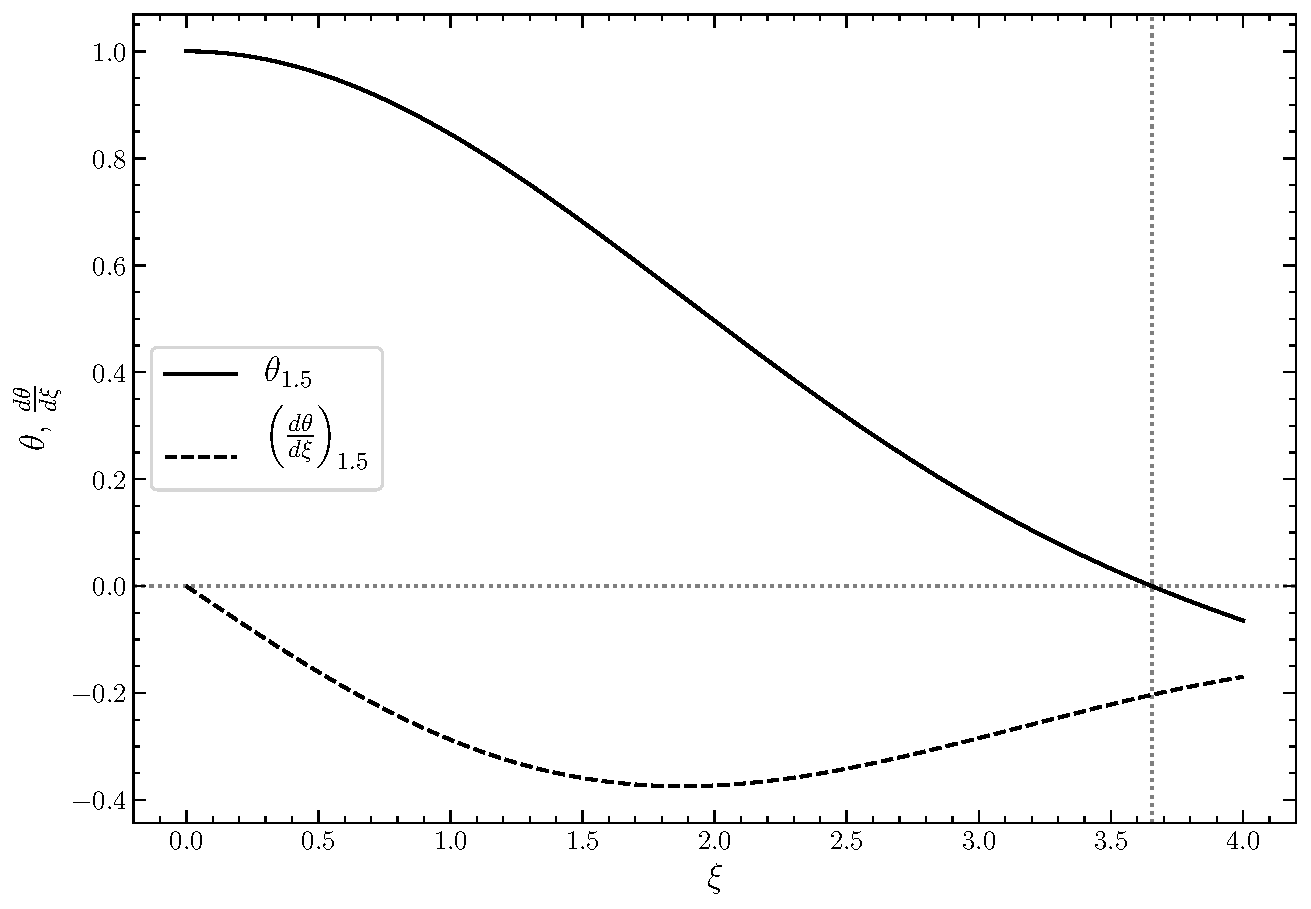
\includegraphics[scale=0.6]{Graphics/ThetaXi.pdf}
    \caption{Solutions for $\theta$ and $d\theta/d\xi$ when $n=1.5$.}
    \label{fig:p2a}
\end{figure}
You can run this using the program \textit{./integrate-nonDegenerate}; refer to the documentation for information on the command line arguments. In order to identify the value of $\theta$ at $\xi_{1}$ I simply find which element in the $\xi$ array corresponds to the minimum absolute value of $\theta$ and define that as $\xi_{1}$. For the case $n=1.5$ I find:
\begin{align*}
    \xi_{1} = 3.65374
\end{align*}

\section{Density Investigation}
Starting from the definition of the total mass
\begin{align*}
    m(r) = \int_{0}^{r}4\pi r^{2}\rho(r)dr
\end{align*}
if we convert into a dimensionless unit system in density
\begin{align*}
    m(r) = 4\pi \rho_{c}\int_{0}^{r}\theta^{n}r^{2}dr
\end{align*}
now we need to convert to a dimensionless unit system in the radial coordinate
\begin{align*}
    m(\xi) = 4\pi\rho_{c}\alpha^{3}\int_{0}^{\xi}\theta^{n}\xi^{2}d\xi
\end{align*}
from the definition of our units we know that $r\equiv\alpha\xi$, so then $\alpha^{3} = \frac{r^{3}}{\xi^{3}}$,
from the Lane-Emden equation we can say that $\int_{0}^{\xi}\theta^{n}\xi^{2}d\xi = -\xi^{2}\frac{d\theta}{d\xi}$
\begin{align*}
    m(\xi) &= -4\pi\rho_{c}\frac{r^{3}}{\xi^{3}}\xi^{2}\frac{d\theta}{d\xi} \\
    m(\xi) &= 4\pi\rho_{c}r^{3}\left[-\frac{1}{\xi}\frac{d\theta}{d\xi}\right]
\end{align*}
now if we look at the total mass $M$ at the surface $r=R$ then
\begin{align*}
    M &= 4\pi\rho_{c}R^{3}\left[-\frac{1}{\xi}\frac{d\theta}{d\xi}\right]_{\xi=\xi_{1}}
\end{align*}
Now if we invoke the definition of average density (that it is the total mass divided by the volume)
\begin{align*}
    \bar{\rho} &= \frac{4\pi\rho_{c}R^{3}\left[-\frac{1}{\xi}\frac{d\theta}{d\xi}\right]_{\xi=\xi_{1}}}{\frac{4}{3}\pi R^{3}} \\
    \bar{\rho} &= 3\rho_{c}\left[-\frac{1}{\xi}\frac{d\theta}{d\xi}\right]_{\xi=\xi_{1}} \\
    \frac{\bar{\rho}}{\rho_{c}} &= \frac{-3}{\xi_{1}}\left[\frac{d\theta}{d\xi}\right]_{\xi=\xi_{1}}
\end{align*}
from here we then solve for $\rho_{c}$
\begin{align*}
    \rho_{c} = -\frac{\bar{\rho}\xi}{3}\left[\frac{d\theta}{d\xi}\right]^{-1}_{\xi=\xi_{1}}
\end{align*}
and now once more we use the definition of the average density
\begin{align*}
    \rho_{c} &= -\frac{M\xi}{3V}\left[\frac{d\theta}{d\xi}\right]^{-1}_{\xi=\xi_{1}} \\
    \rho_{c} &= -\frac{M\xi}{3\frac{4}{3}\pi R^{3}}\left[\frac{d\theta}{d\xi}\right]^{-1}_{\xi=\xi_{1}} \\
    \rho_{c} &= -\frac{M\xi}{4\pi R^{3}}\left[\frac{d\theta}{d\xi}\right]^{-1}_{\xi=\xi_{1}}
\end{align*}

\section{Relations to Physical Quantities}
From numerical integration of the Lane-Emden equation we can find $\xi_{1}$ and $\frac{d\theta}{d\xi}$ this then lets us find the ratio of the average to central pressure. 
\begin{align*}
    \frac{\bar{\rho}}{\rho_{c}} = -\frac{3}{\xi_{1}}\left(\frac{d\theta}{d\xi}\right)_{\xi=\xi_{1}}
\end{align*}
We know $M$ and $R$ so we can find $\bar{\rho}$ as that is simply
\begin{align*}
    \bar{\rho} &= \frac{3M}{4\pi R^{3}}
\end{align*}
then using $\xi$ and $d\theta/d\xi$ we can find the central density using
\begin{align*}
    \rho_{c} &= -\frac{\bar{\rho}\xi_{1}}{3}\left(\frac{d\theta}{d\xi}\right)_{\xi=\xi_{1}}^{-1} \\
    \rho_{c} &= -\frac{M\xi_{1}}{4\pi R^{3}}\left(\frac{d\theta}{d\xi}\right)_{\xi=\xi_{1}}^{-1}
\end{align*}
So now we can find the run of density as a function of $\theta$
\begin{align*}
    \rho &= \rho_{c}\theta^{n} \\
    \rho &= -\frac{M\xi_{1}\theta^{n}}{4\pi R^{3}}\left(\frac{d\theta}{d\xi}\right)_{\xi=\xi_{1}}^{-1}
\end{align*}
In order to find $P$ and $T$ we first use the known values of $\xi_{1}$ and $R$ to find $\alpha$
\begin{align*}
    R &= \alpha \xi_{1} \\
    \alpha &= \frac{R}{\xi_{1}}
\end{align*}
We can find the value $K$ from the definition of the total mass
\begin{align*}
    M = -\frac{1}{\sqrt{4\pi}}\left[\frac{K(n+1)}{G}\right]^{3/2}\rho_{c}^{(3-n)/2n}\left[\xi^{2}\frac{d\theta}{d\xi}\right]_{\xi_{1}}
\end{align*}
Now we solve for $K$ in terms of $M$
\begin{align*}
    K^{3/2} &= \frac{M\sqrt{4\pi}G^{3/2}}{\xi^{2}_{1}(n+1)^{3/2}\rho_{c}^{(3-n)/2n}}\left(-\frac{d\theta}{d\xi}\right)_{\xi_{1}}^{-1} \\
    K &= \left[\frac{M\sqrt{4\pi}G^{3/2}}{\xi^{2}_{1}(n+1)^{3/2}\rho_{c}^{(3-n)/2n}}\left(-\frac{d\theta}{d\xi}\right)_{\xi_{1}}^{-1}\right]^{2/3} \\
    K &= \frac{M^{2/3}2^{2/3}\pi^{1/3}G}{\xi^{4/3}_{1}(n+1)\rho_{c}^{(3-n)/3n}}\left(-\frac{d\theta}{d\xi}\right)_{\xi_{1}}^{-2/3}
\end{align*}
Using $K$ we can get the run of pressure from the polytropic equation of state
\begin{align*}
    P = K\rho_{c}^{1+1/n}\theta^{n+1}
\end{align*}
Finally, we can use the given equation of state to get the temperature run
\begin{align*}
    P &= \frac{k\rho T}{\mu m_{p}}\\
    T &= \frac{P\mu m_{p}}{k\rho}
\end{align*}
We have all the components of this, so we have solved for $T$.

\section{Scaling Numeric Solution to Physical Quantities}
Using the relations derived in \S 5 I scale the solution found from numeric integration in \S 3. Firstly, both the total mass and total radius are needed a-priori. The problem statement gives the mass in parts \textit{a} and \textit{b} as $1$ M$_{\odot}$ and in part \textit{c} as $1.3$ M$_{\odot}$.  Additionally, if we make the assumption that the star is well approximated as a black body then the given luminosity and effective temperature constrain the radius through the Stephan-Boltzmann equation
\begin{align*}
    L &= 4\pi\sigma R^{2}T^{4} \\
    R &= \sqrt{\frac{L}{4\pi\sigma^{2}T^{4}}}
\end{align*}
where $\sigma$ is the Stephan-Boltzmann constant. The luminosity is given in log solar units, so we must first convert the given value of $\log(L/L_{\odot})=1.5$ to cgs units.
\begin{align*}
    \log(\frac{L}{L_{\odot}}) &= 1.5 \\
    \frac{L}{L_{\odot}} &= 10^{1.5} \\
    L &= 10^{1.5}L_{\odot}
\end{align*}
so then the radius is given as
\begin{align*}
    R &= \sqrt{\frac{10^{1.5}L_{\odot}}{4\pi\sigma^{2}4000\text{[K]}}}
\end{align*}
Using the provided code base the script \textit{pyUtils/convertToPhysical.py} will allow one to scale the general numeric solution to physical quantities. For the three given situations (Solar Composition at Solar Mass, Big Bang Composition at Solar Mass, and Solar Composition at 1.3 Solar Masses) I find the physical solutions given in Figure \ref{fig:physical}.

\begin{figure}
    \centering
    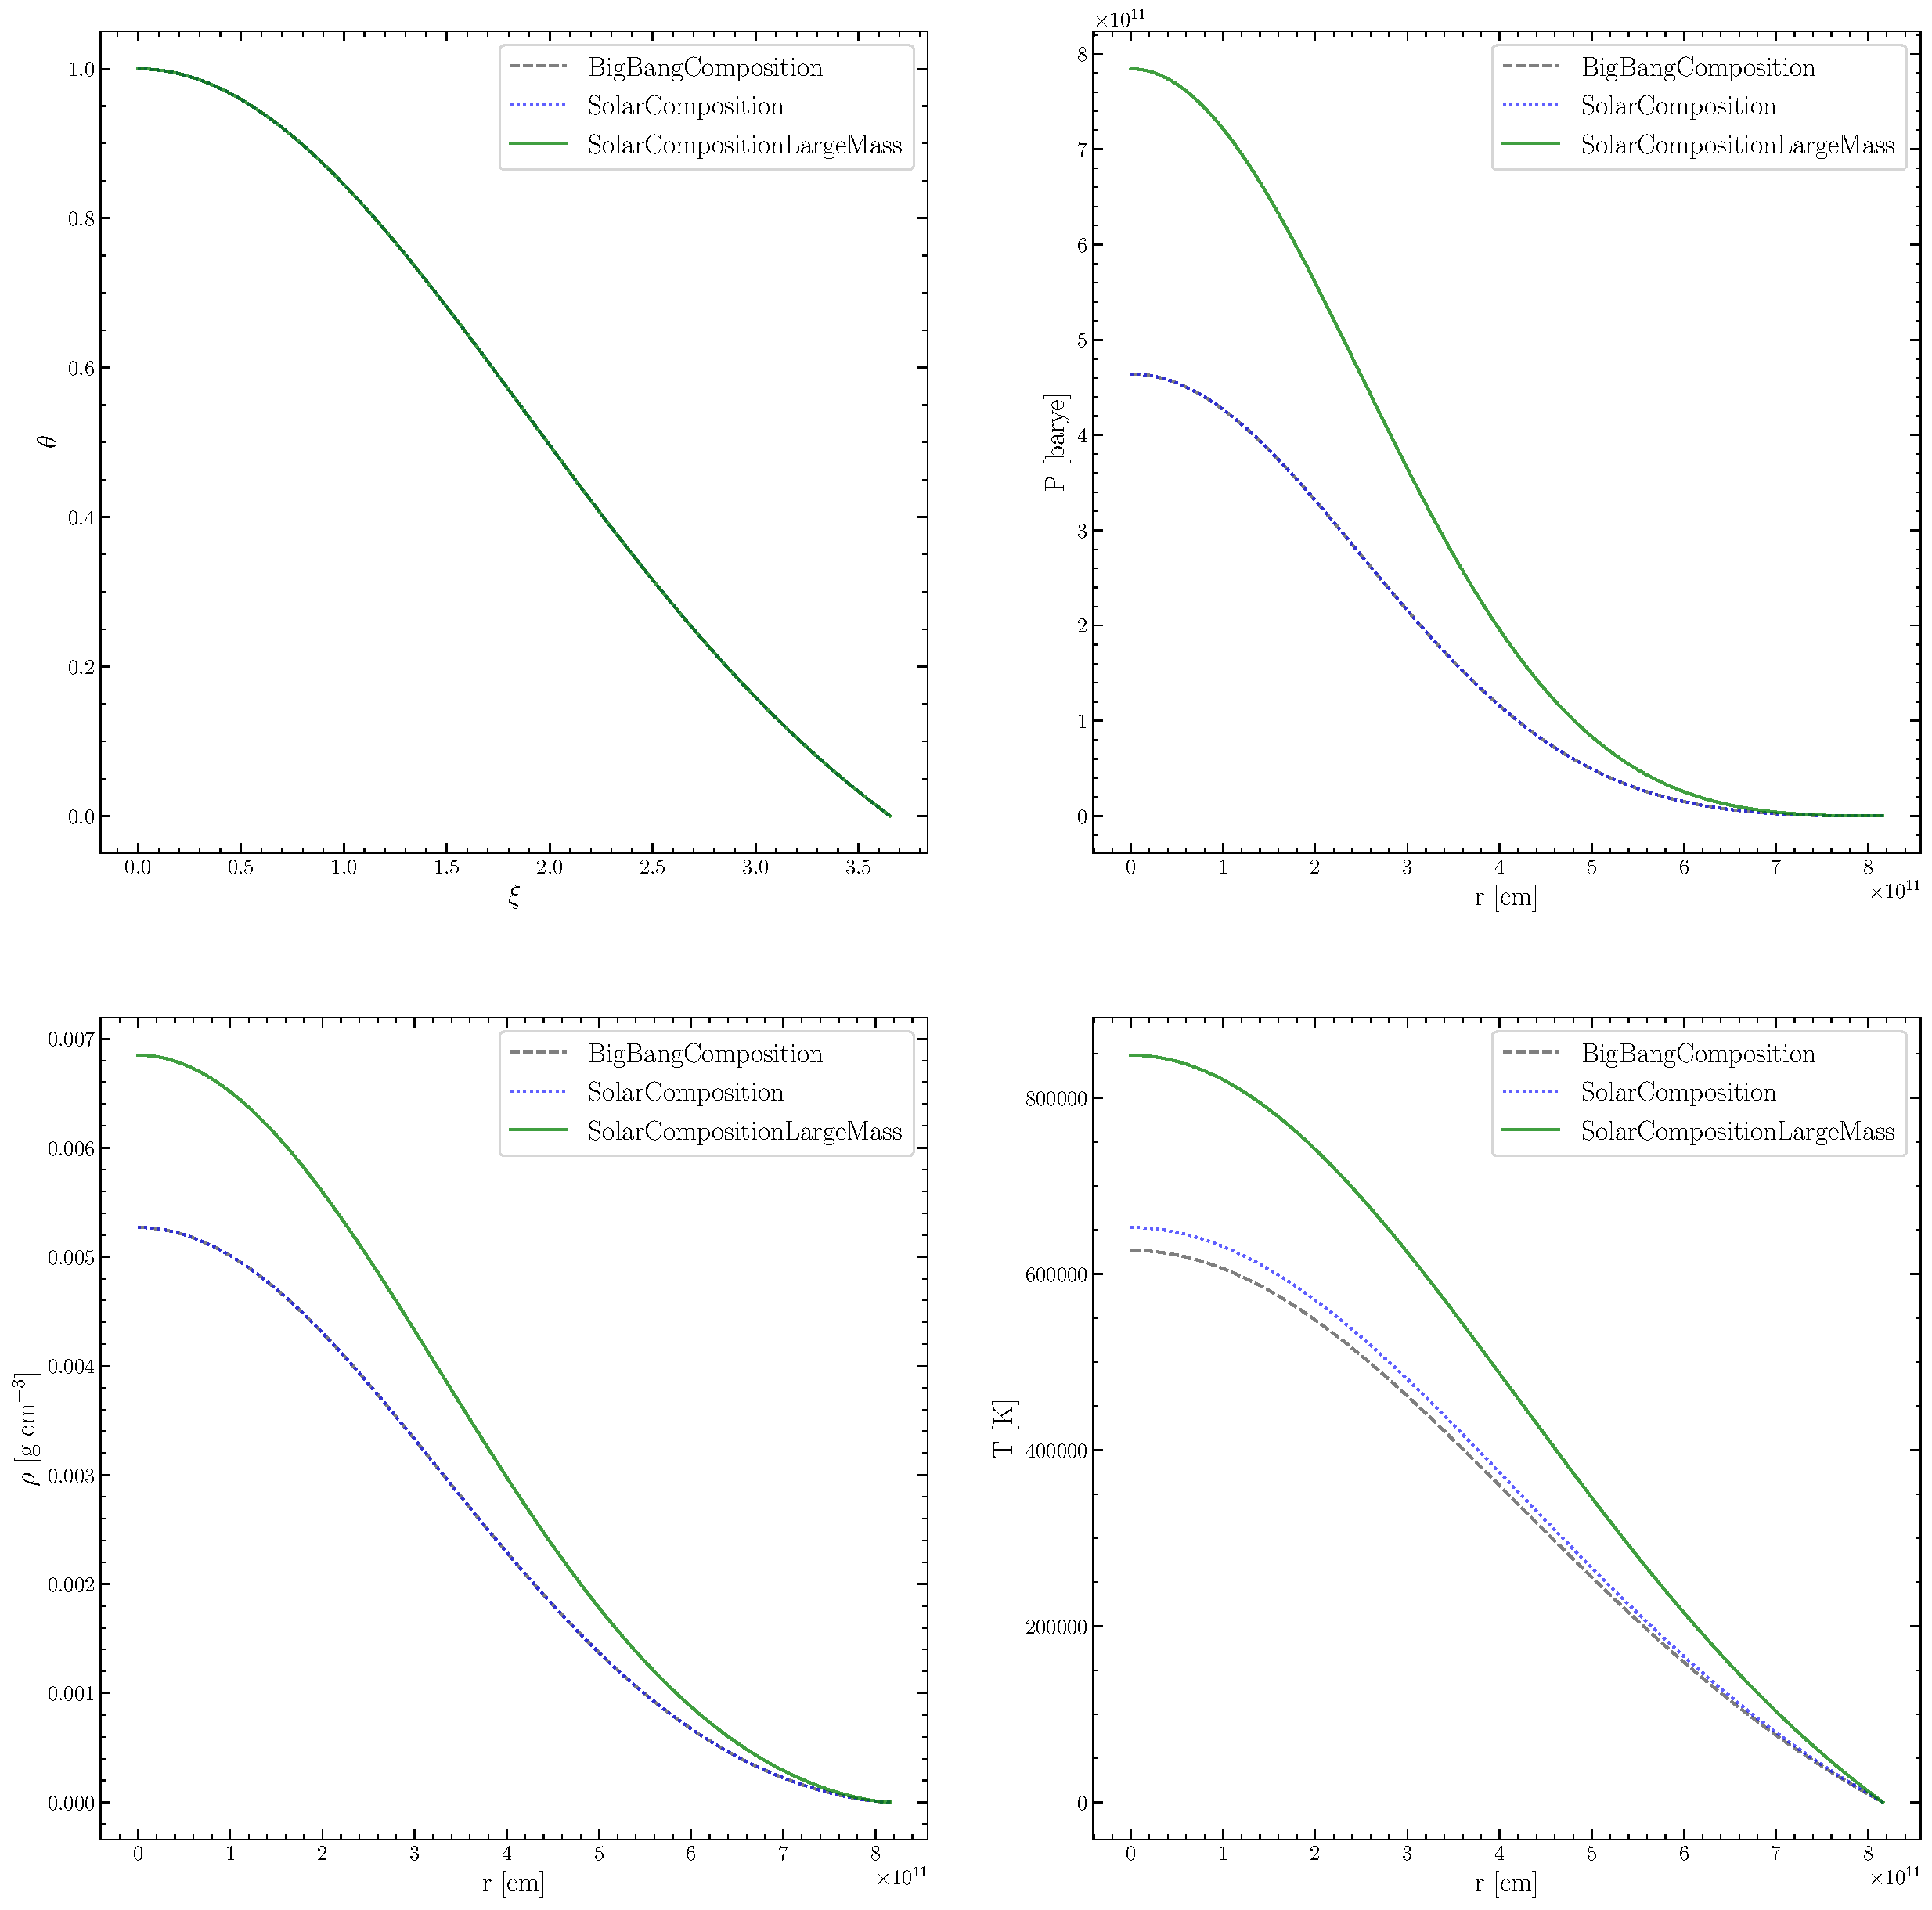
\includegraphics[width=\textwidth]{Graphics/AllCompositions.pdf}
    \caption{Physical Solutions for three different situations. Note that in the upper left graph there will be no difference between scaled solutions as that is a graph of the pre--scaled values. Additionally, note that in the case of density and pressure the solutions of equal mass but varied composition lie on top of each other.}
    \label{fig:physical}
\end{figure}

\textbf{(a). Solar Composition at One Solar Mass:} At one solar mass we find a central temperature of $8\pt{5}$ [K]. This is about 5 percent of the sun's central temperature; however, this lower value is consistent with $n=1.5$ modeling a pre-main sequence star as the central temperature should be low enough that hydrogen fusion can not yet ignite. Similarly, the central density is approximately four orders of magnitude lower than the sun's central density and six orders of magnitude lower than the sun's central pressure.

\textbf{(b). Big Bang Composition:} Holding the mass and the radius constant, but varying the composition of the stellar model changes only the temperature profile, lowering the average temperature compared to a current solar composition model. This difference arise from a change in the average molecular mass, $\mu$, which will alter the temperature profile due to its place in the ideal gas equation of state.

\textbf{(c). Solar Composition at 1.3 Solar Masses:} By Keeping the composition the same but increasing the mass the average density changes. This change in the average density propagates through to all other quantities, increasing their average values. Therefore the density, pressure, and temperature all have higher average values for the higher mass solar composition case. One interesting note is that the relative difference in pressure between the one and 1.3 solar mass case is much larger than the relative change in density and temperature. 

\section{White Dwarf Structure}
The problem given is that:
\begin{align*}
    P \equiv \frac{P_{N}P_{R}}{\sqrt{P_{N}^{2}+P_{R}^{2}}}
\end{align*}
Additionally, we are given that
\begin{align*}
    P_{N} &= K_{N}\rho^{5/3} \\
    P_{R} &= K_{N}\rho^{5/3} \\
    \rho_{0} &= \left(\frac{K_{R}}{K_{N}}\right)^{3}
\end{align*}
so then plugging these into the given equivalency
\begin{align*}
    P &= \frac{K_{N}\rho^{5/3}K_{R}\rho^{4/3}}{\sqrt{(K_{N}\rho^{5/3})^{2}+(K_{R}\rho^{4/3})^{2}}} \\
    P &= \frac{K_{N}\rho^{5/3}K_{R}\rho^{4/3}}{\sqrt{K_{N}^{2}\rho^{10/3}+K_{R}^{2}\rho^{8/3}}} \\
    P &= \frac{K_{N}\rho^{5/3}K_{R}\rho^{4/3}}{\rho^{4/3}\sqrt{K_{N}^{2}\rho^{2/3}+K_{R}^{2}}} \\
    P &= \frac{K_{N}\rho^{5/3}K_{R}}{\sqrt{K_{N}^{2}\rho^{2/3}+K_{R}^{2}}} \\
    P &= \frac{K_{N}\rho^{5/3}K_{R}}{K_{R}\sqrt{\frac{K_{N}^{2}}{K_{R}^{2}}\rho^{2/3}+1}} \\
% \end{align*}
% \begin{align*}
     P &= \frac{K_{N}\rho^{5/3}}{\sqrt{\frac{K_{N}^{2}}{K_{R}^{2}}\rho^{2/3}+1}} \\
     P &= \frac{K_{N}\rho^{5/3}}{\sqrt{\frac{1}{\rho^{2/3}_{0}}\rho^{2/3}+1}} \\
     P &= \frac{K_{N}\rho^{5/3}}{\sqrt{\frac{\rho^{2/3}}{\rho^{2/3}_{0}}+1}}
\end{align*}

\section{Quantum Gas Equations of States}
Plotting the Equations from the previous section we find the solutions shown in Figure \ref{fig:degFG}.
\begin{figure}
    \centering
    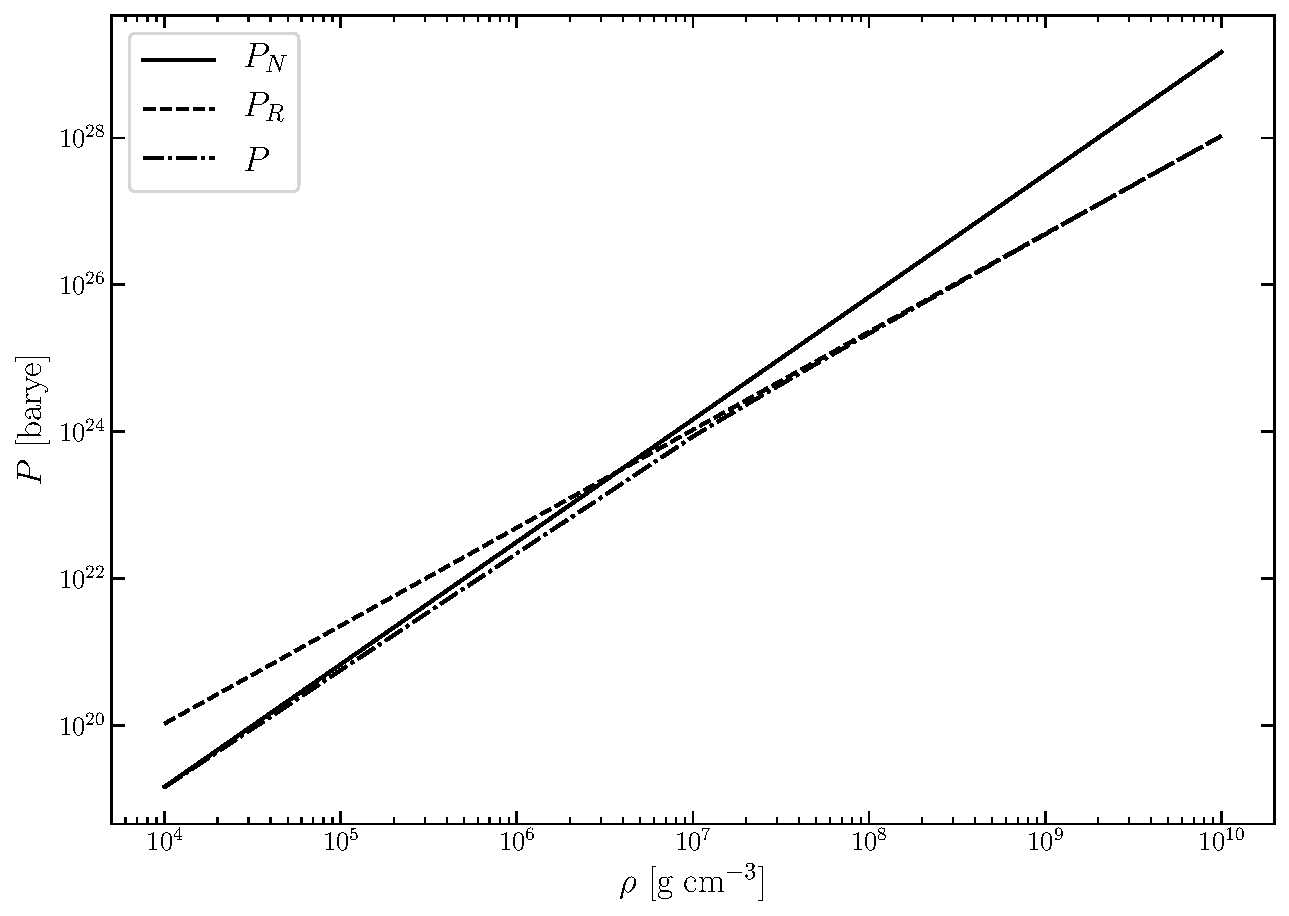
\includegraphics[width=0.75\textwidth]{Graphics/FermiEOS.pdf}
    \caption{Three equations of state for a degenerate Fermi gas}
    \label{fig:degFG}
\end{figure}
We can see from Figure \ref{fig:degFG} that the combined equation of state well approximates the non-relativistic solution for low densities and the relativistic solutions at high densities. More problematic is the transition region between these two states, around a million grams per cubic centimeter, where the merged equation of state approximates neither well. Therefore, in the case where a degenerate Fermi gas is either essentially all relativistic (high densities) or all non- relativistic (low densities) the merged equation will provide a valid approximation; in the case where one needs to transition between the two states the merged solution will diverge from both equations of states. This may be physical appropriate; however, it is outside the scope of this project to determine that.

\section{Structure Equation for a White Dwarf}
If we start with the equations of hydrostatic equilibrium and mass continuity
\begin{align*}
    \frac{dP}{dr} &= -\frac{Gm\rho}{r^{2}}\\
    \frac{dm}{dr} &= \rho4\pi r^{2}
\end{align*}
we can slightly rearrange the equation of hydrostatic equilibrium
\begin{align*}
    \frac{1}{\rho}\frac{dP}{dr} &= -\frac{Gm}{r^{2}}
\end{align*}
if we take another derivative wrt. $r$, applying the product rule as we do, so given than both $r$ and $m$ are dependent on $r$, 
\begin{align*}
    \frac{d}{dr}\left(\frac{1}{\rho}\frac{dP}{dr}\right) &= \frac{2Gm}{r^{3}} - \frac{G}{r^{2}}\frac{dm}{dr} 
\end{align*}
we can now substitute in for the mass differential using the equation of mass continuity
\begin{align*}
    \frac{d}{dr}\left(\frac{1}{\rho}\frac{dP}{dr}\right) &= \frac{2Gm}{r^{3}} - \frac{G}{r^{2}}\rho4\pi r^{2} \\
    \frac{d}{dr}\left(\frac{1}{\rho}\frac{dP}{dr}\right) &= \frac{2Gm}{r^{3}} - 4\pi G\rho
\end{align*}
Moreover, we can recognize that we can implant another pressure differential into the first term on the right using the equation of hydrostatic equilibrium
\begin{align*}
    \frac{d}{dr}\left(\frac{1}{\rho}\frac{dP}{dr}\right) &= -\frac{2r}{\rho}\frac{dP}{dr} - 4\pi G\rho 
\end{align*}
Moving terms around such that they may be further simplified
\begin{align*}
    \frac{d}{dr}\left(\frac{1}{\rho}\frac{dP}{dr}\right) + \frac{2r}{\rho}\frac{dP}{dr} &=  - 4\pi G\rho 
\end{align*}
if we multiply the equation by $r^{2}$ then the left side of the equation is simply the result of applying a product rule differential with respect to $r$, if we undo that operation
\begin{align*}
    \frac{d}{dr}\left(\frac{r^{2}}{\rho}\frac{dP}{dr}\right) &=  - 4\pi G\rho r^{2} \\
    \frac{1}{r^{2}}\frac{d}{dr}\left(\frac{r^{2}}{\rho}\frac{dP}{dr}\right) &=  - 4\pi G\rho
\end{align*}
we now have something which looks very much like the Lane-Emden equation. Note that to this point nothing we have done is specific to any equation of state or definition of dimensionless parameters. If we now let $\rho=\rho_{0}\theta$ and let $P=K_{N}\rho_{0}^{5/3}\theta^{5/3}(1+\theta^{2/3})^{-1/2}$ then
\begin{align*}
    \frac{1}{r^{2}}\frac{d}{dr}\left(\frac{r^{2}}{\rho_{0}\theta}\frac{d}{dr}\left[K_{N}\rho_{0}^{5/3}\theta^{5/3}(1+\theta^{2/3})^{-1/2}\right]\right) &= -4\pi G\rho_{0}\theta
\end{align*}
pulling out all the non $r$ dependent terms from the derivative
\begin{align*}
    \frac{K_{N}\rho_{0}^{5/3}}{\rho_{0}^{2}4\pi G}\frac{1}{r^{2}}\frac{d}{dr}\left(\frac{r^{2}}{\theta}\frac{d}{dr}\left[\theta^{5/3}(1+\theta^{2/3})^{-1/2}\right]\right) &= -\theta
\end{align*}
we know there is some constant $\alpha$ such that $r\equiv \alpha \xi$. Let us define then 
\begin{align*}
    \alpha^{2} \equiv \frac{K_{N}\rho_{0}^{5/3}}{\rho_{0}^{2}4\pi G} \\
    \alpha^{2} \equiv \frac{K_{N}}{4\pi G\rho_{0}^{1/3}}
\end{align*}
if we take a side bar to evaluate this numerically then we find that
\begin{align*}
    \alpha &= 0.00223456 R_{\odot}
\end{align*}
then back to finding the Lane-Emden-like equation 
\begin{align*}
       \alpha^{2}\frac{1}{r^{2}}\frac{d}{dr}\left(\frac{r^{2}}{\theta}\frac{d}{dr}\left[\theta^{5/3}(1+\theta^{2/3})^{-1/2}\right]\right) &= -\theta
\end{align*}
if we replace $r=\alpha\xi$ and $dr=\alpha d\xi$ then
\begin{align*}
    \alpha^{2}\frac{1}{\alpha^{2}\xi^{2}}\frac{1}{\alpha}\frac{d}{d\xi}\left(\frac{\alpha^{2}\xi^{2}}{\theta}\frac{1}{\alpha}\frac{d}{d\xi}\left[\theta^{5/3}(1+\theta^{2/3})^{-1/2}\right]\right) &= -\theta
\end{align*}
because $\alpha$ is a constant it can be pulled out of the differential. If we do that we will find that $\alpha$ cancels to 1, so then we arrive at the form given in the question
\begin{align*}
   \frac{1}{\xi^{2}}\frac{d}{d\xi}\left(\frac{\xi^{2}}{\theta}\frac{d}{d\xi}\left[\theta^{5/3}(1+\theta^{2/3})^{-1/2}\right]\right) &= -\theta
\end{align*}
We can then break this down into two coupled first order differential equations. To start I use Mathematica to expand the left side
{\small
\begin{align*}
    -\theta = \frac{3 \xi  \theta \left(4 \theta^{4/3}+9 \theta^{2/3}+5\right) \theta''+\theta
   '\left(6 \theta\left(4 \theta^{4/3}+9 \theta^{2/3}+5\right)-\xi  \left(8
   \theta^{2/3} \left(\theta^{2/3}+2\right)+5\right) \theta'\right)}{9 \xi\left(\theta^{2/3}+1\right)^{5/2} \theta^{4/3}}
\end{align*}}
Now if we let $\nu\equiv \frac{d\theta}{d\xi}$ then
{\small
\begin{align*}
    -\theta = \frac{3 \xi \theta \left(4 \theta^{4/3}+9 \theta^{2/3}+5\right) \nu'+\nu\left(6 \theta\left(4 \theta^{4/3}+9 \theta^{2/3}+5\right)-\xi \left(8
   \theta^{2/3} \left(\theta^{2/3}+2\right)+5\right) \nu\right)}{9 \xi\left(\theta^{2/3}+1\right)^{5/2} \theta^{4/3}}
\end{align*}}
Then, using Mathematica I solve for $\nu'$
{\small
\begin{align*}
    \nu' = \frac{-6 \left(\theta^{2/3}+1\right) \left(4 \theta^{2/3}+5\right) \theta \nu+\xi\left(8 \theta^{2/3} \left(\theta^{2/3}+2\right)+5\right) \nu^2-9 \xi  \left(\theta^{2/3}+1\right)^{3/2} \theta^3-9 \xi  \left(\theta^{2/3}+1\right)^{3/2} \theta^{7/3}}{3 \xi  \left(\theta^{2/3}+1\right) \left(4 \theta^{2/3}+5\right) \theta}
\end{align*}}
if we simplify this and break into separate terms
\begin{align*}
    \nu' = -\frac{2\nu}{\xi} + \frac{\xi\left(8 \theta^{2/3} \left(\theta^{2/3}+2\right)+5\right) \nu^2-9 \xi  \left(\theta^{2/3}+1\right)^{3/2} \theta^3-9 \xi  \left(\theta^{2/3}+1\right)^{3/2} \theta^{7/3}}{3 \xi  \left(\theta^{2/3}+1\right) \left(4 \theta^{2/3}+5\right) \theta}
\end{align*}
At this point the algebra is pretty ugly but there are a few important things to note. In general form this is the same as what is given, i.e you can break it into three terms, one with no $\nu$ dependency, one with a linear dependence and one with a quadratic dependence on $\nu$. So instead of manipulating it until it works, I simply use Mathematica to divide what I have by what is given in the project. When I do this Mathematica returns a 1. Using the "That's how fractions work" Theorem I deduce that when x/y = 1 $x$ and $y$ are the same thing. Therefore what I have above is equivalent to what is given in the project.

\section{Numerical Integration -- Degenerate Case}
Using the two given coupled first order differential equations I create a new "degenerate" integrator (using the same integration scheme as in the non--degenerate case). You can use this integrator by running the program \textit{./integrate-degenerate}. See the documentation for details on the command line arguments. I create with a log scale of densities\footnote{\scriptsize \$ python -c "import numpy as np; print('\textbackslash n'.join([str(x) for x in np.logspace(-3, 5, 20)]))" > run\_of\_theta.dat} ranging from $10^{-3}$ to $10^{5}$, which I then generate numeric solutions for\footnote{\$ cat run\_of\_theta.dat | xargs -I\{\} ./integrate-degenerate \{\} 0.00001 0.00001 12}.

\section{Analyzing White Dwarf Integration}
\subsection{Mass -- Central Density}
I first plot on a log linear linear scale the mass vs the central density of 20 white dwarf models (Figure \ref{fig:WDmass}). I fit a slightly generalized logistic function of the form
\begin{align*}
    f(x, a, b, c) = \frac{a}{1+e^{-(cx-b)}}
\end{align*}
using a non-linear least squares fitting routine\footnote{scipy.optimize.curve\_fit} and extract one sigma errors from the covarience matrix. I find a best fit value for the maximum stable mass of $a=1.46\pm0.001$ M$_{\odot}$. Incidentally this section also serves as the test case for the validity of my WD integrator, given that we know that the maximum expected WD mass is $\sim$1.44 M$_{\odot}$ and I find something very near to that.
\begin{figure}[ht!]
    \centering
    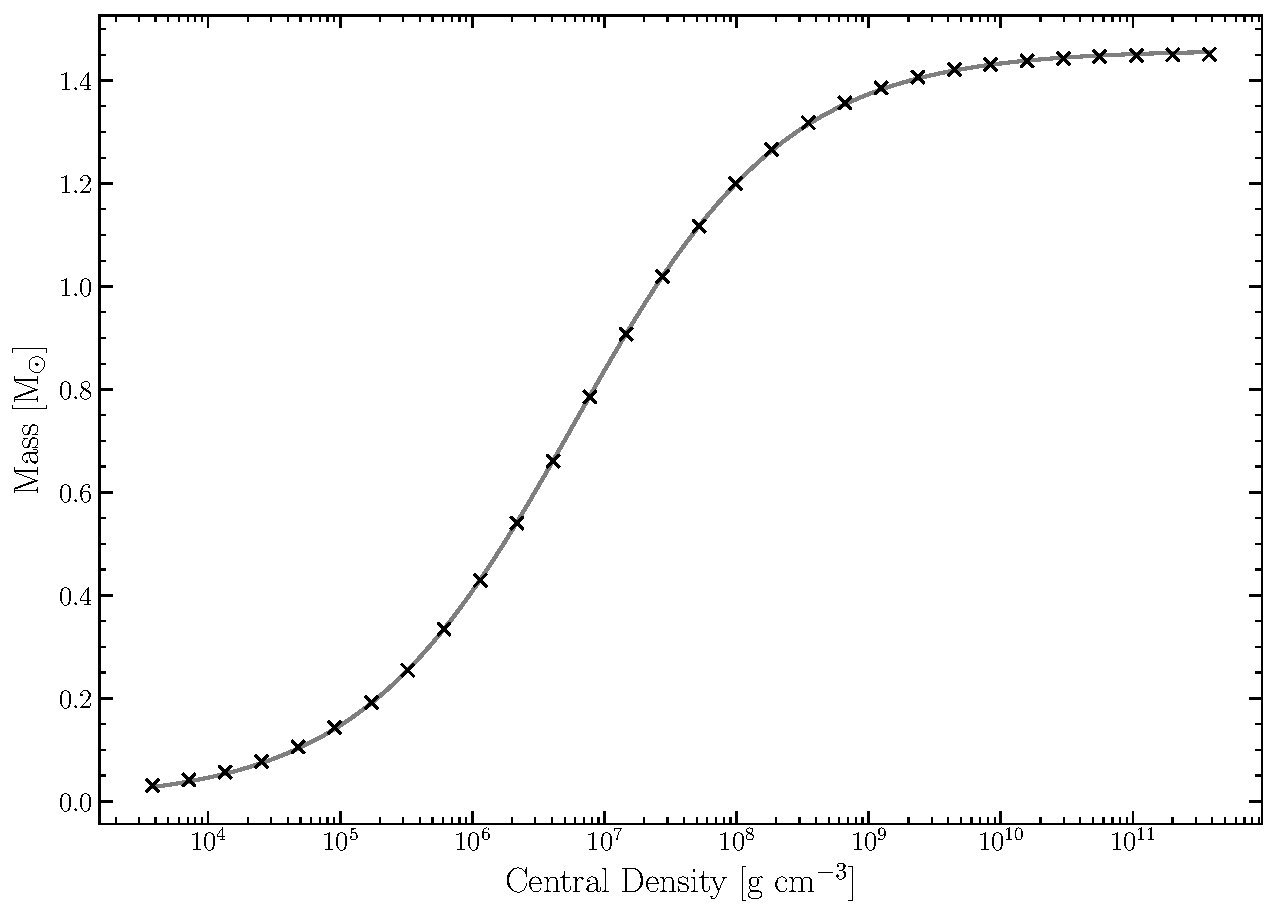
\includegraphics[width=0.75\textwidth]{Graphics/WDMasses.pdf}
    \caption{Total Mass vs. Central Density of degenerate model with logistic function fit to determine asymptote. I find a max stable mass of 1.46 M$_{\odot}$.}
    \label{fig:WDmass}
\end{figure}
\subsection{Radius -- Central Density}
When we look at how the radius varies with the central density we find Figure \ref{fig:WDRRho}.
\begin{figure}[ht!]
    \centering
    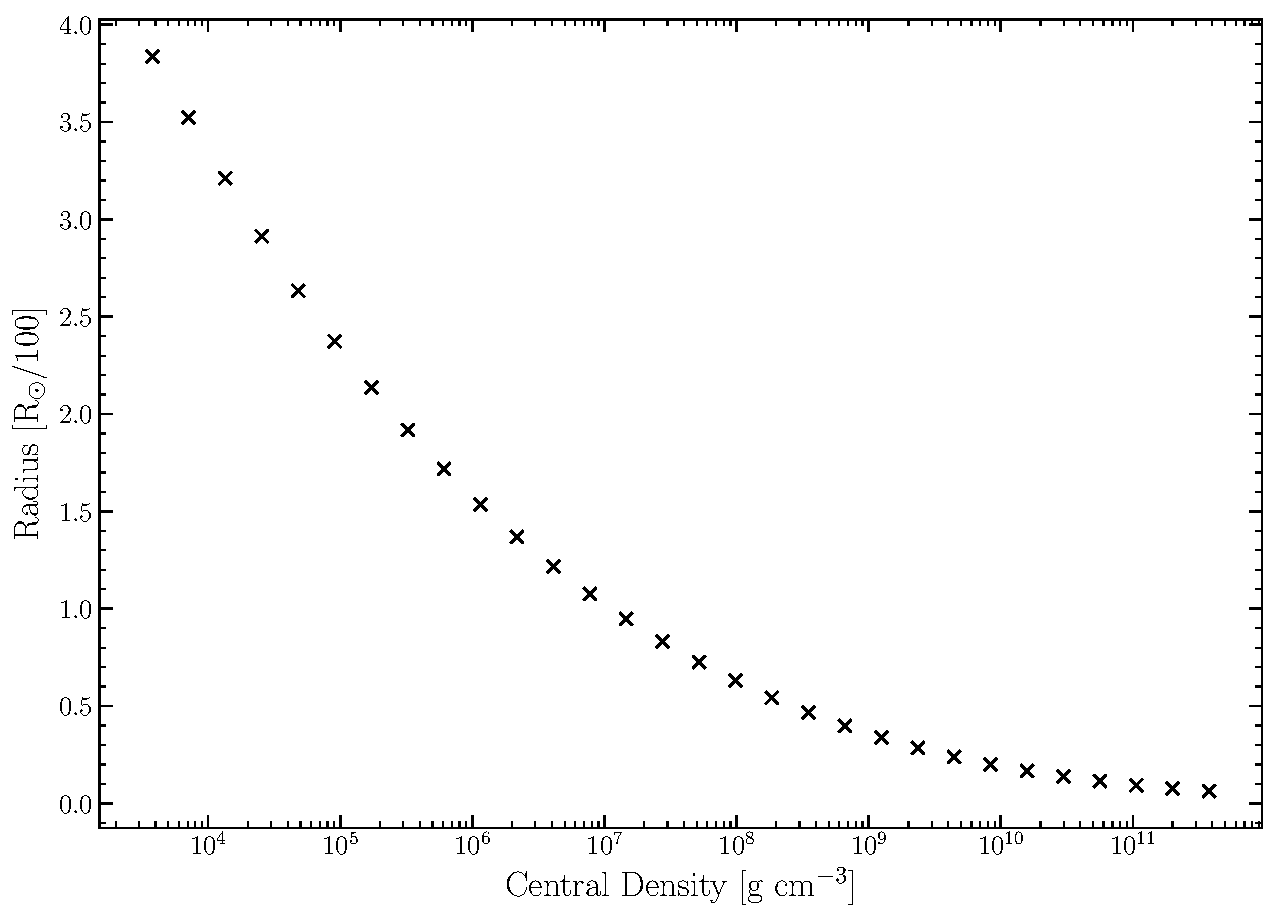
\includegraphics[width=0.75\textwidth]{Graphics/WD_R_Rho.pdf}
    \caption{The run of total radius as central density is varied.}
    \label{fig:WDRRho}
\end{figure}
\subsection{Mass -- Radius for the Degenerate Case}
Next we can look at the relation between mass and total radius of the WD (Figure \ref{fig:WDMR}). The mass radius relation makes the degenerate nature of WD clear, as as the mass increases the radius decreases.
\begin{figure}[ht!]
    \centering
    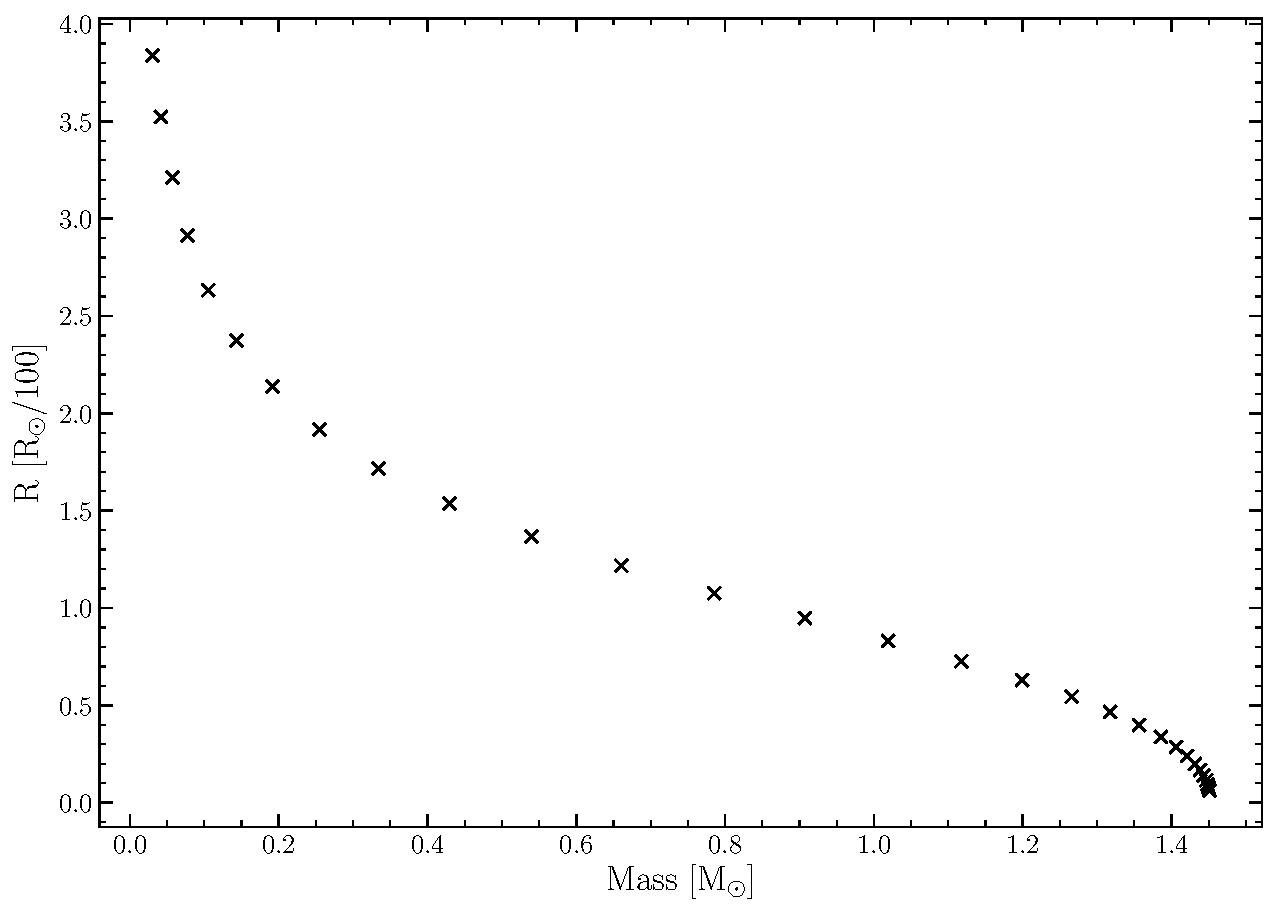
\includegraphics[width=0.75\textwidth]{Graphics/WD_M_R.pdf}
    \caption{Mass Radius Relation of the WD model presented in this project.}
    \label{fig:WDMR}
\end{figure}
\subsection{Mass -- Radius Relation for the Non--Degenerate Case}
For this final case we find Figure \ref{fig:TwoWDMass} showing the run of density to radial position in the star.
\begin{figure}[ht!]
    \centering
    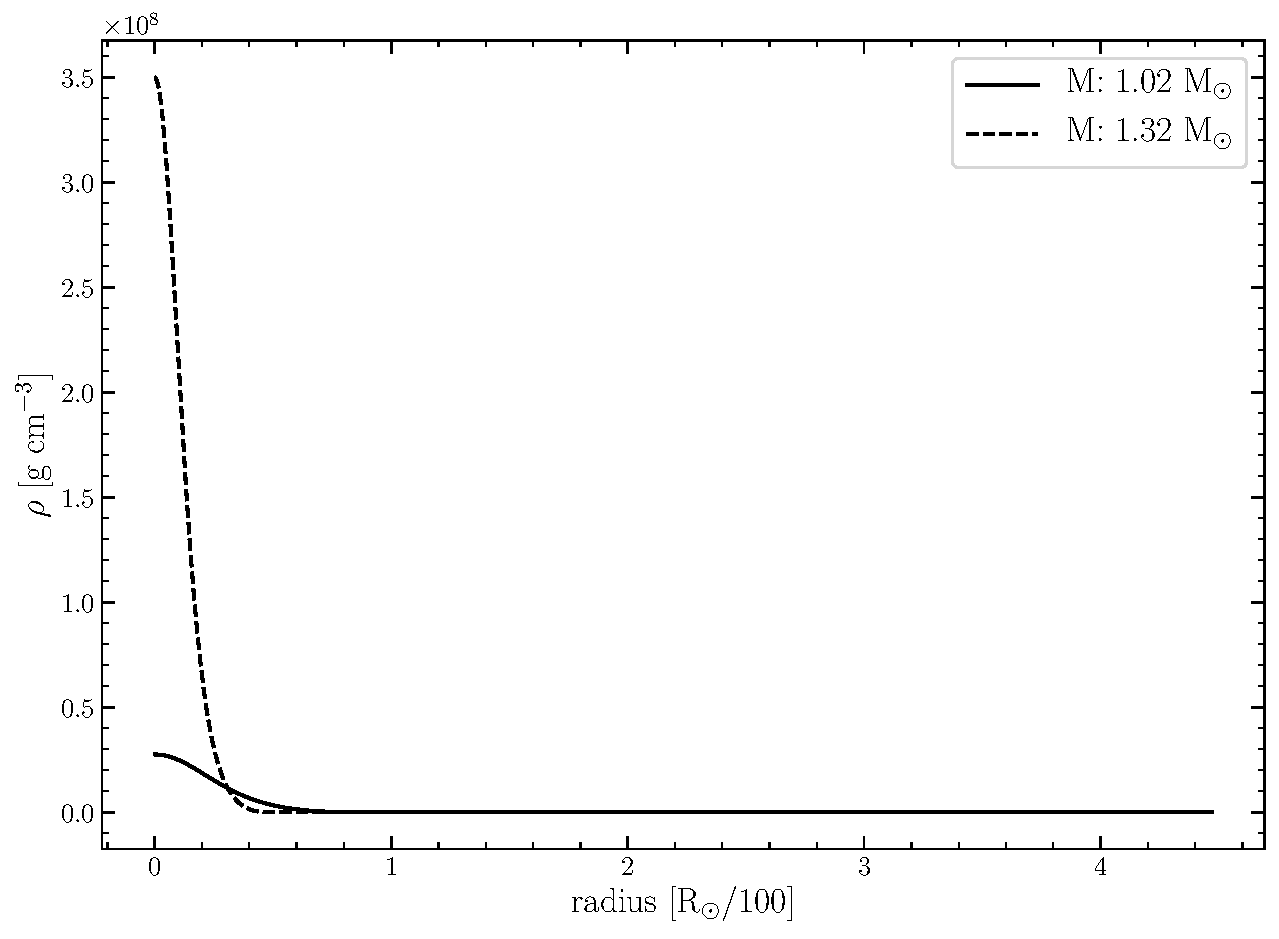
\includegraphics[width=0.75\textwidth]{Graphics/WDMass1_13.pdf}
    \caption{Density vs. Radius for two WD models. Note how the WD model of larger mass has a density which goes to zero faster than the other model.}
    \label{fig:TwoWDMass}
\end{figure}

% \bibliographystyle{unsrt}
% \bibliography{ms}

\end{document}
